\chapter{Literature Review}\label{cha:literature}

    % TODO: Some other intro

\section{State of the Art}

    % TODO: some intro

    \subsection{ROS on Web}

        The closest representation of the intended project is the work produced by Michael Allwright known as \textit{ROS on Web}. Allwright shares the same goal as the author to develop the technology which allows for running ROS nodes entirely on the browser by cross-compiling C++ code to WebAssembly and using web workers to handle the internal communication~\cite{rosonweb}.

        Equivalently, Allwright targeted the \ac{ROS} 2 distribution. It is suspected that the \textit{galactic} version was used for the demonstrations. The main demonstration of a running publisher and subscriber is illustrated in Figure~\ref{fig:rosweb}.
        
        
        \begin{figure}[htbp]
            \centering
            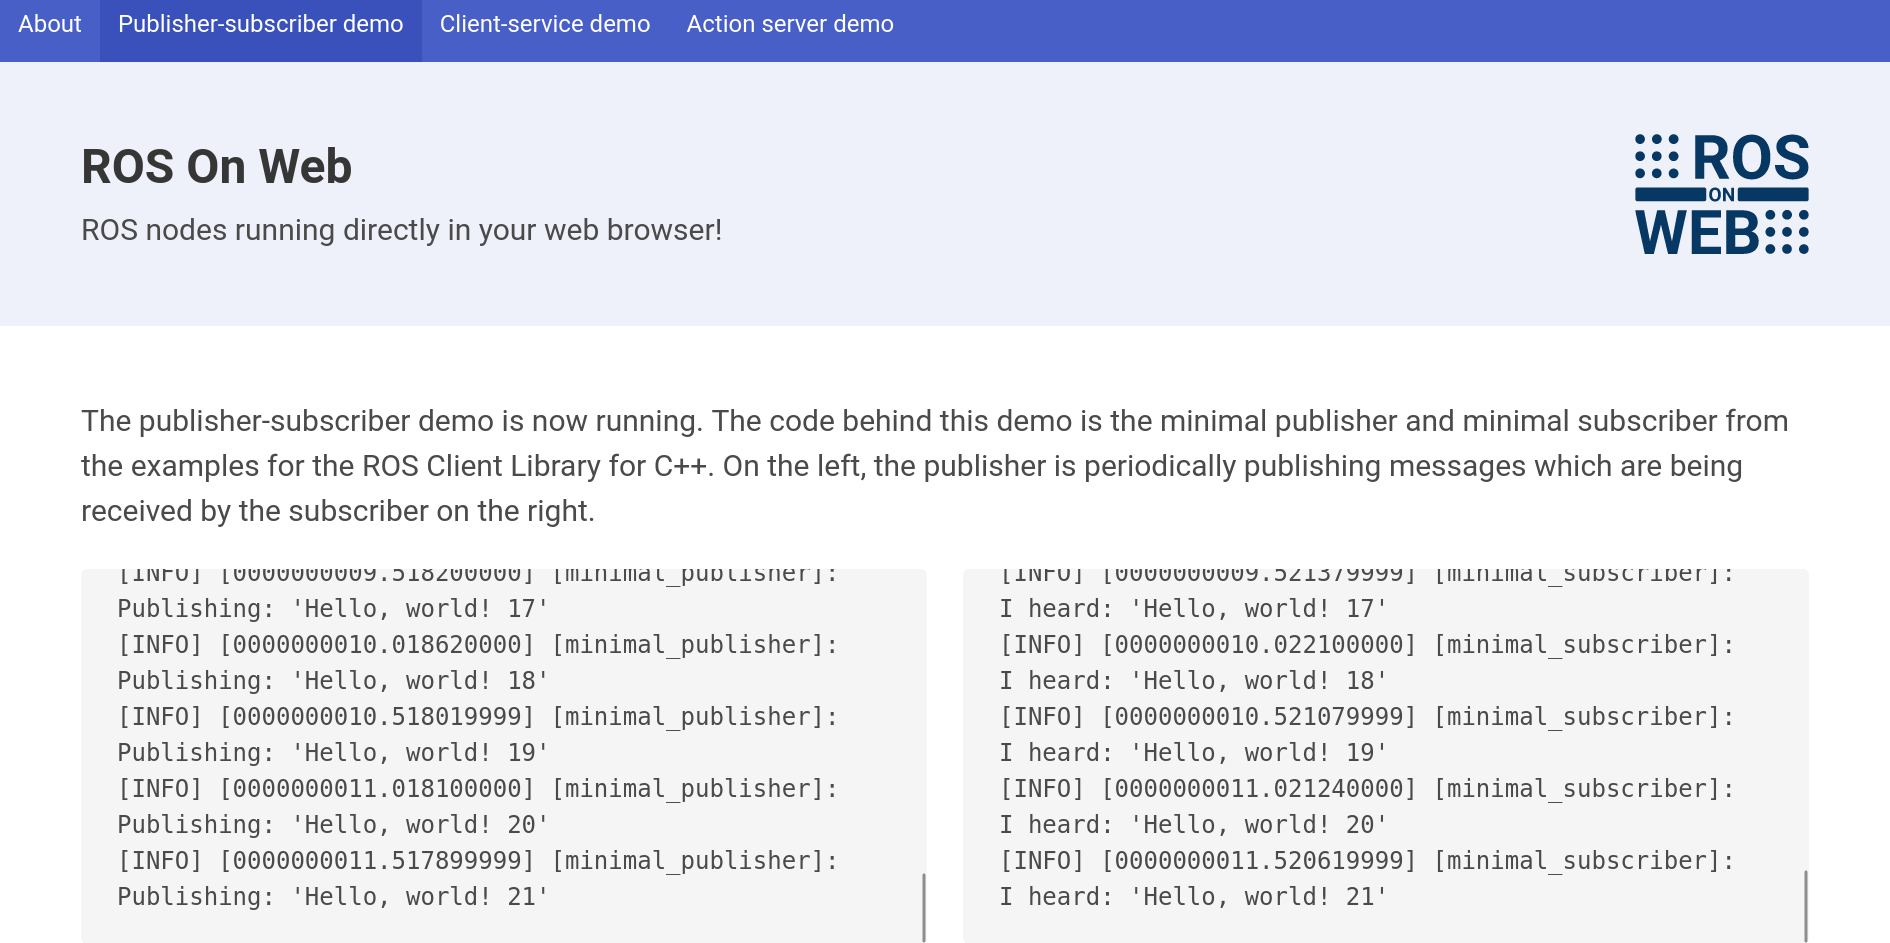
\includegraphics[width=\textwidth]{01_rosOnWeb.png}
            \caption{\textit{ROS on Web} publisher and subscriber demonstration.}
            \label{fig:rosweb}
        \end{figure}

        Nonetheless, the greatest disadvantage of \textit{ROS on Web} lies in the fact that the project is not open source. Very little can be derived about how Allwright was able to achieve the demonstrations represented on the website. A few hints are given in the introductory page such as the replacement of the middleware with a custom design and the use of web workers. However, it is not possible to determine the manner in which these technologies were used. Hope remains that in the near future, the repositories for \textit{ROS on Web} become publicly available as an extension of the ROS open source ecosystem.

    \subsection{roswasm\_suite}

        Another project closely related to the author's developments is \textsf{roswasm\_suite} currently maintained mainly by Nils Bore. This suite is a set of libraries which help the user to cross\-compile C++ ROS nodes to WebAssembly~\cite{roswasmsuite}. It also includes a library of helpers to write web \ac{GUI}s for ROS; one such example can be observed in Figure~\ref{fig:roswasm_gui}.

        \begin{figure}[htbp]
            \centering
            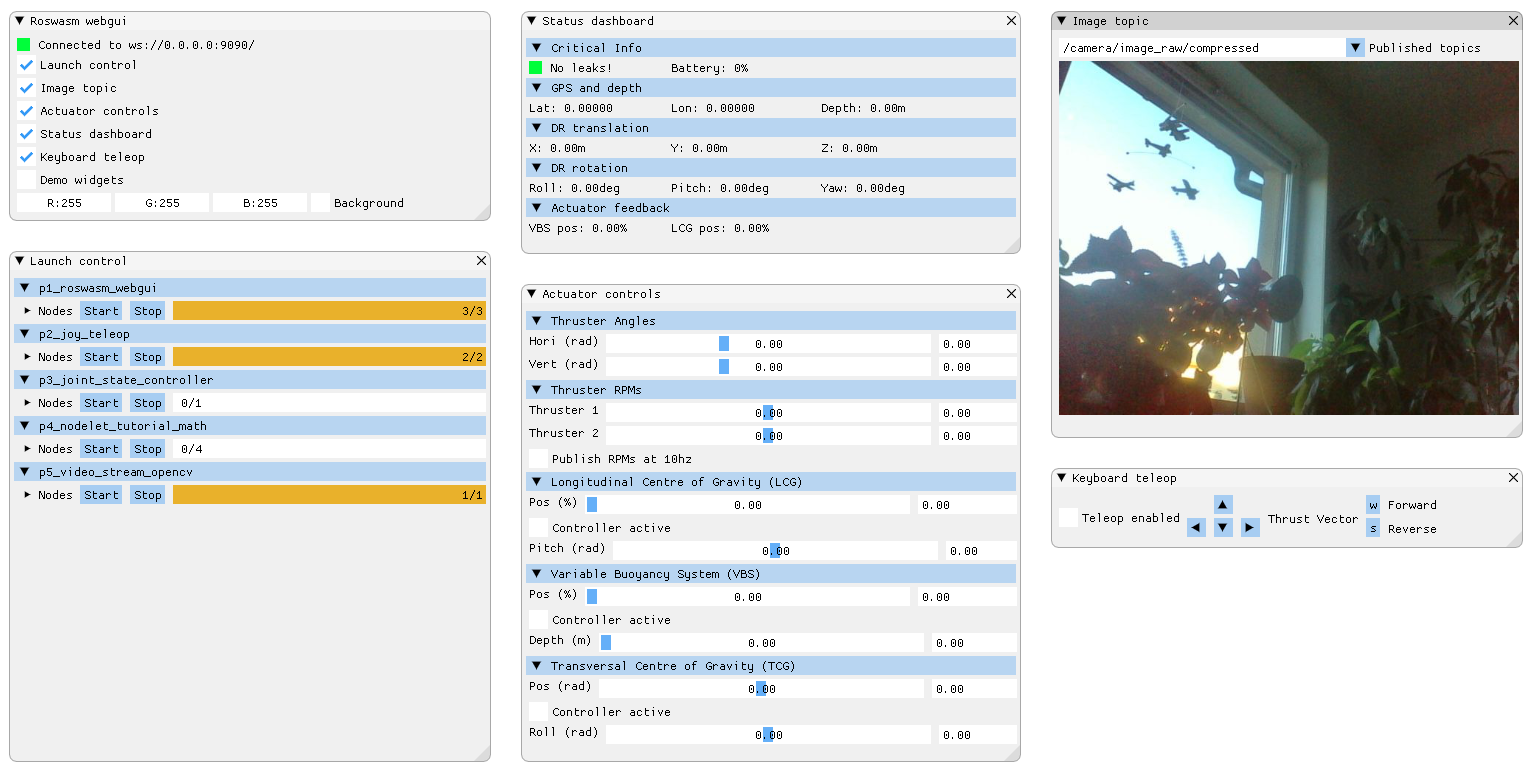
\includegraphics[width=\textwidth]{01_roswasm_gui.png}
            \caption{Example \ac{GUI} for ROS using \textsf{roswasm\_gui}.}
            \label{fig:roswasm_gui}
        \end{figure}

        Some of the biggest advantages of this \textsf{roswasm\_suite} are that it is open source and actively maintained. The developers have a long history of continuous improvements to the packages, and as of 2023, they have managed to publish ten releases. 

        Nevertheless, these libraries do come with their set of disadvantages. First, the suite targets a \ac{ROS} 1 distro and it depends on \textsf{catkin} tools to build the packages. Thus, the user is required to have a \ac{ROS} 1 installation and the Emscripten \ac{SDK} before being able to use these libraries to launch \ac{ROS} nodes on the browser.


\section{Relevant Works}

    There are several other works which do not directly align with the goals for this project but pertinent in regards to the idea of developing a robotics environment which can be used on a web browser.

    \subsection{Foxglove Studio}

        One of the most notorious examples of robotics applications on the browser consists of Foxglove Studio.
        
        % https://foxglove.dev/blog/publishing-and-visualizing-ros2-transforms
        \begin{figure}[htbp]
            \centering
            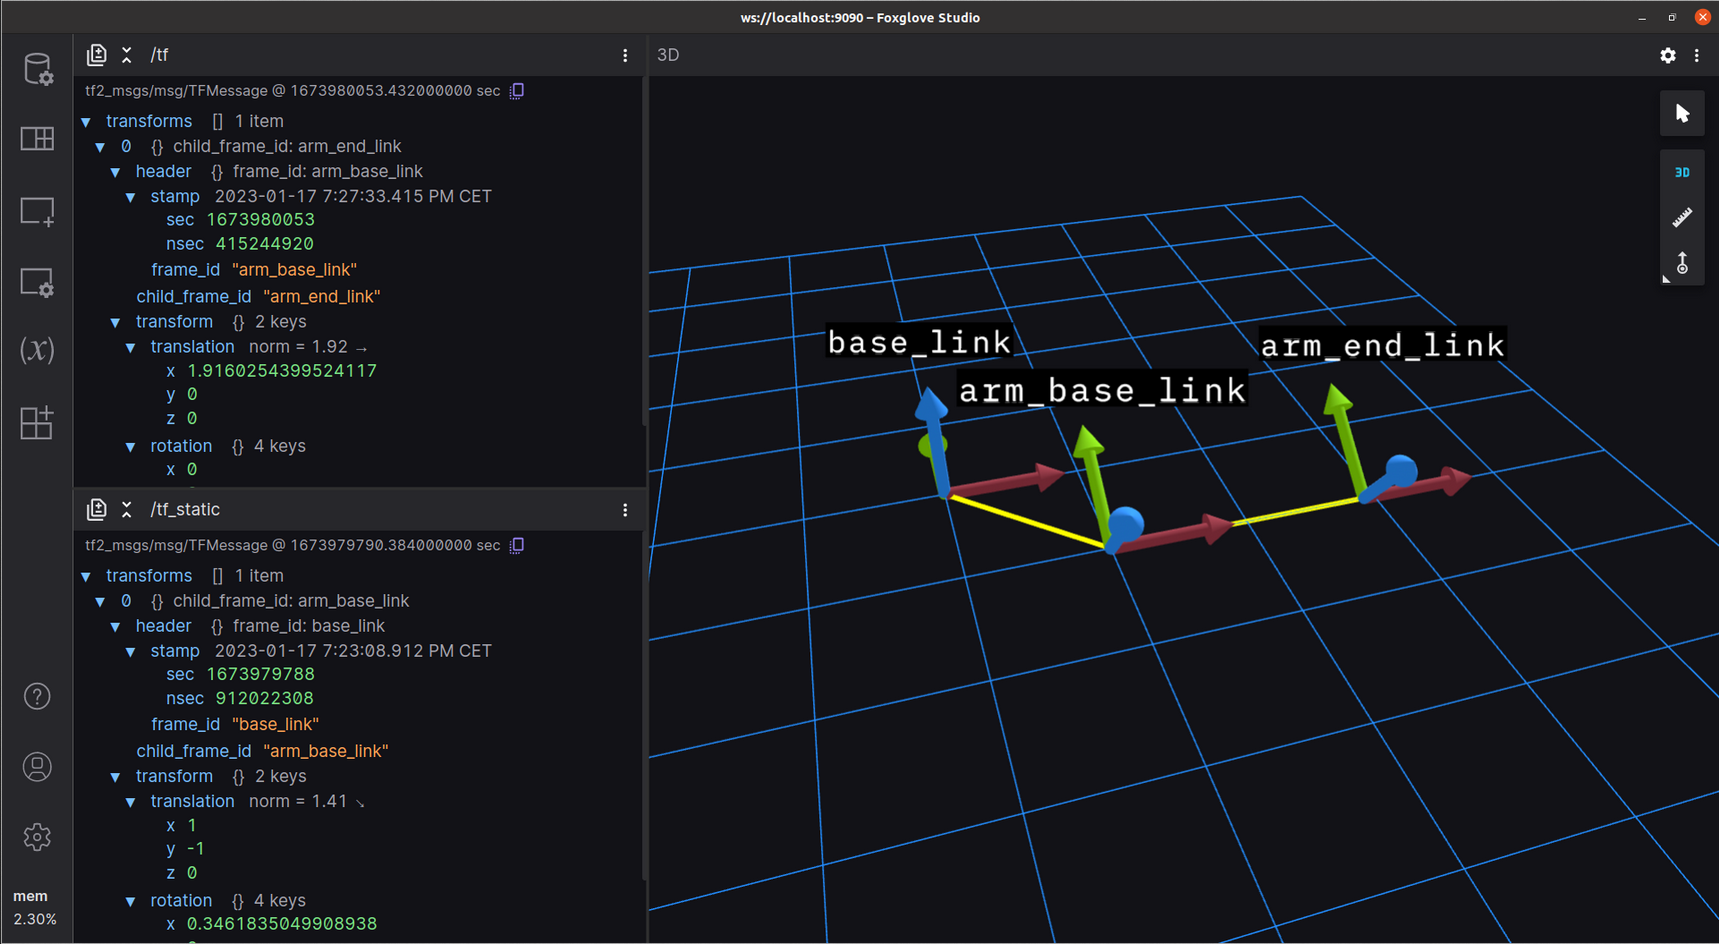
\includegraphics[width=\textwidth]{01_FoxgloveStudio.png}
            \caption{Visualizing ROS 2 Transforms with Foxglove Studio}
        \end{figure}

        \subsection{ROSbridge}

    \subsection{ROS Control Center}

    \subsection{ROSboard}

    \subsection{ROSlink}

\section{State of WASM}

    \subsection{Unity in WebAssembly}

    % https://blog.unity.com/technology/webassembly-is-here
    % https://beta.unity3d.com/jonas/AngryBots/

    \begin{figure}[htbp]
        \centering
        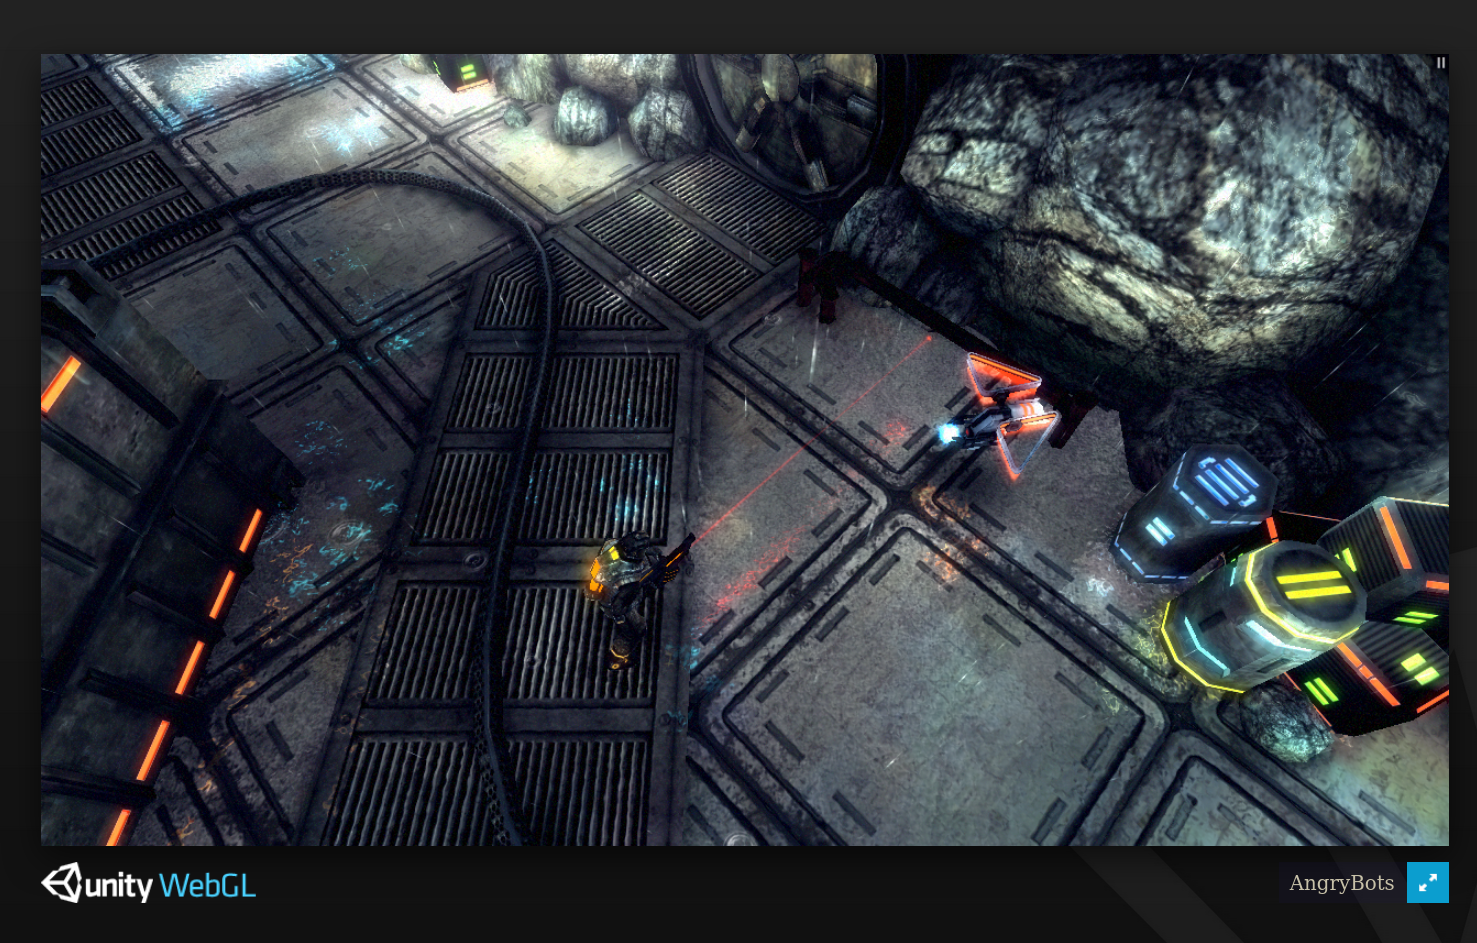
\includegraphics[width=0.8\textwidth]{01_angryBots.png}
        \caption{Demo of Angry Bots in Unity WebGL}\label{fig:unity}
    \end{figure}
